\documentclass[11pt, oneside]{article}
\usepackage[margin=1in]{geometry}
\usepackage{setspace}
\usepackage{amsmath}
\usepackage{amsfonts}
\usepackage{amsthm}
\usepackage{amssymb}
\usepackage{mparhack}
\usepackage{commath}
\usepackage[ddmmyy]{datetime}
\allowdisplaybreaks
\newcommand{\mymarginpar}[1]{\marginpar{\setstretch{1}\textit{\scriptsize{#1}}}}
\newcounter{lecture}
\newcommand{\lecture}[5][]{%
  \addtocounter{lecture}{1}%
  \newdate{@date\arabic{lecture}}{#3}{#4}{#5}%
  \mymarginpar{Lecture \arabic{lecture}\\\displaydate{@date\arabic{lecture}}\\(#2 hour)}
  }

\usepackage[pagebackref]{hyperref}
\hypersetup{
    colorlinks,
    citecolor=black,
    filecolor=black,
    linkcolor=black,
    urlcolor=black
}
  
\renewcommand{\vec}[1]{\mathbf{#1}}
\newcommand{\uvec}[1]{\vec{\hat{#1}}}

\usepackage{tikz}
\usetikzlibrary{arrows,positioning} 
\tikzset{
    %Define standard arrow tip
    >=stealth',
    %Define style for boxes
    punkt/.style={
           rectangle,
           rounded corners,
           draw=black, very thick,
           text width=6.5em,
           minimum height=2em,
           text centered},
    % Define arrow style
    pil/.style={
           ->,
           thick,
           shorten <=2pt,
           shorten >=2pt,}
}

\begin{document}
\title{\textbf{Revision Notes for AE2-209 Mathematics}}
\author{Vishnu R Menon\\ 
\small{Department of Aeronautics, Imperial College London}}

\maketitle
\tableofcontents

\newpage

\section{Vector Space}
\lecture{1}{09}{10}{2017}
\subsection{Cartesian Coordinates}
If a vector $\vec{a}$ is three-dimensional,

\begin{equation}
\vec{a} \in \mathbb{R}^3  
\end{equation}
where,
\begin{equation}
a_1,a_2,a_3 \in \mathbb{R}
\end{equation}
\subsection{Cylindrical Coordinates}
\lecture{1}{10}{10}{2017}
\begin{align}
  x&=rcos(\theta)\\
  y&=rsin(\theta)\\
  z&=z
\end{align}

\subsection{Spherical Coordinates}
\begin{align}
  x&=rcos(\theta)sin(\phi)\\
  y&=rsin(\theta)sin(\phi)\\
  z&=z
\end{align}


\subsection{Norm: Length of Vector}
For $\vec{a} \in \mathbb{R}^3$, 
\begin{equation}
  \norm{\vec{a}}\equiv\sqrt{\vec{a}\cdot\vec{a}}=\sqrt{a_1^2+a_2^2+a_3^2}
\end{equation}
Distance between 2 points, $\vec{a}$, $\vec{b}$ is
\begin{equation}
  \norm{\vec{a}-\vec{b}}=\sqrt{(a_1-b_1)^2+(a_2-b_2)^2+(a_3-b_3)^2}
\end{equation}


\subsection{Inner Product}
%For $\vec{a}$, $\vec{b} \in \mathbb{R}^3$, i.e. $\vec{a} = (a_1,a_2,a_3)$, $\vec{b} = (b_1,b_2,b_3)$
\begin{equation}
\vec{a} \cdot \vec{b}=\sum_{i=1}^3 a_ib_i = a_1b_1 + a_2b_2 + a_3b_3
\end{equation}
\begin{equation}
  \vec{a} \cdot \vec{b} = \norm{\vec{a}} \norm{\vec{b}} cos(\theta)
\end{equation}
where $\theta$ is the acute angle between $\vec{a}$ and $\vec{b}$.

\subsubsection{Properties of Inner Product}

%For $\vec{a}$, $\vec{b}$, $\vec{c} \in \mathbb{R}^3$ and $\alpha$, $\beta \in \mathbb{R}$,

\begin{enumerate}
  \item \begin{align}
    \vec{a}\cdot\vec{a}&\geq0\\
    \vec{a}\cdot\vec{a}&=0 \text{ (if and only if } \vec{a} = 0)
  \end{align}
  
  \item Associative (wrt. scalar multiplication)
  \begin{equation}
    (\alpha\vec{a})\cdot\vec{b} = \alpha(\vec{a}\cdot\vec{b})
  \end{equation}
  \item Distributive
  \begin{align}
    \vec{a}\cdot(\vec{b}+\vec{c}) &= \vec{a}\cdot\vec{b} + \vec{a}\cdot\vec{c}\\
    (\vec{a}+\vec{b})\cdot\vec{c} &= \vec{a}\cdot\vec{c} + \vec{b}\cdot\vec{c}
  \end{align}
  \item Commutative
  \begin{equation}
    \vec{a}\cdot\vec{b} = \vec{b}\cdot\vec{a}
  \end{equation}
  \item Orthogonal\\
  Two non-zero vectors, $\vec{a}$ and $\vec{b}$ are orthoganal if and only if,
  \begin{equation}
    \vec{a}\cdot\vec{b} = 0
  \end{equation}
\end{enumerate} 

\subsubsection{Cauchy-Schwartz Inequality}
\begin{equation}
  \abs{\vec{a}\cdot\vec{b}}\leq\norm{\vec{a}} \norm{\vec{b}}
\end{equation}

\begin{proof}
  \begin{align}
    \vec{a}\cdot\vec{b} &= \norm{\vec{a}} \norm{\vec{b}} cos(\theta)\\
    \abs{\vec{a}\cdot\vec{b}} &= \abs{\norm{\vec{a}}  \norm{\vec{b}}cos(\theta)}\\
    \abs{\cos(\theta)} &\leq 1\\
    \abs{\vec{a}\cdot\vec{b}}&\leq\norm{\vec{a}} \norm{\vec{b}}
  \end{align}
\end{proof}

\subsubsection{Triangle Inequality}
\begin{equation}
  \norm{\vec{a}+\vec{b}} \leq \norm{\vec{a}}+\norm{\vec{b}}
\end{equation}
\begin{proof}
  \begin{align}
    LHS: \norm{\vec{a}+\vec{b}}^2 &= (\vec{a}+\vec{b})\cdot(\vec{a}+\vec{b})\\
    &= \norm{\vec{a}}^2 + 2\vec{a}\cdot\vec{b} + \norm{\vec{b}}^2\\
    RHS: (\norm{\vec{a}}+\norm{\vec{b}})^2 &= \norm{\vec{a}^2}+ 2\norm{\vec{a}}\norm{\vec{b}} +\norm{\vec{b}^2}\\
    \because \abs{\vec{a}\cdot\vec{b}}&\leq\norm{\vec{a}} \norm{\vec{b}} \text{(Cauchy-Schwartz Inequality)}\\
    \therefore \norm{\vec{a}}^2 + 2\vec{a}\cdot\vec{b} + \norm{\vec{b}}^2 &\leq \norm{\vec{a}^2}+ 2\norm{\vec{a}}\norm{\vec{b}} +\norm{\vec{b}^2}\\
    \norm{\vec{a}+\vec{b}} &\leq \norm{\vec{a}}+\norm{\vec{b}}
  \end{align}
\end{proof}
\subsection{Cross Product}
\lecture{1}{12}{10}{2017}
\begin{align}
  \vec{a}\times\vec{b}&=det \begin{bmatrix}
       \vec{i} & \vec{j} & \vec{k}          \\[0.3em]
       a_1  & a_2 & a_3 \\[0.3em]
       b_1  & b_2 & b_3     \end{bmatrix}\\
       &= (a_2b_3-a_3b_2)\vec{i} + (a_3b_1-a_1b_3)\vec{j} + (a_1b_2-a_2b_1)\vec{k}\\
       &= \norm{\vec{a}}\norm{\vec{b}}sin(\theta)
\end{align}
\subsubsection{Properties of Cross Product}
\begin{enumerate}
  \item Anti-commutative\begin{equation}
 \vec{a}  \times\vec{b}=-\vec{b}\times\vec{a}
 \end{equation}
 \item Distributive \begin{align}
    \vec{a}\times(\alpha\vec{b}+\beta\vec{c}) &= \alpha(\vec{a}\times\vec{b}) + \beta(\vec{a}\times\vec{c})\\
    (\alpha\vec{a}+\beta\vec{b})\times\vec{c} &= \alpha(\vec{a}\times\vec{c}) + \beta(\vec{b}\times\vec{c})
  \end{align}
\item Cyclic Permutation
  \begin{eqnarray}
    \vec{i}\times\vec{j}=\vec{k} &\vec{j}\times\vec{k}=\vec{i} &\vec{k}\times\vec{i}=\vec{j}
  \end{eqnarray}
\begin{figure}[!h]
\centering

  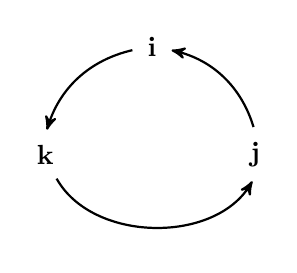
\begin{tikzpicture}[node distance=1cm, auto,]

 \node[] (dummy) {};
 \node[right=of dummy] (j) {$\vec{j}$};
 \node[left=of dummy] (k) {$\vec{k}$}
   edge[pil, bend right=60] (j.south);
  \node[above=of dummy] (i) {$\vec{i}$}
    edge[pil,<-,bend left=30] (j.north)
    edge[pil, bend right=30] (k.north);
\end{tikzpicture}
\end{figure}

\end{enumerate}

\subsubsection{Curve(path)}
Let $\vec{r}:\mathbb{R} \rightarrow \mathbb{R}^3$ and $t \in \mathbb{R}$. A curve C is then defined such that
\begin{equation}
  \vec{r}(t) = (x(t),y(t),z(t))
\end{equation}
where t is called a parameter of the curve and a tangent vector to the curve at $\vec{r}(t)$ is given by
\begin{equation}
  \frac{d\vec{r}(t)}{dt}=\bigg(\frac{dx(t)}{dt},\frac{dy(t)}{dt},\frac{dz(t)}{dt}\bigg)
\end{equation}

\section{Differentiation of Scalar-Valued Function}
\lecture{1}{13}{10}{2017}
\subsection{Scalar-Valued Function}
A map, \textbf{domain of which is multi-dimensional} and the \textbf{range of which is one dimensional}, is called a scalar-valued function, i.e.
\begin{equation}
f:\mathbb{R}^n \rightarrow \mathbb{R} \quad \text{for n $\geq 1$}
\end{equation}

\subsection{Level Set}

Let $f:\mathbb{R}^n \rightarrow \mathbb{R}$ and $c \in \mathbb{R}$. Then, the \textbf{level set value} of $c$ is defined to be the all the points of $\vec{x} \in \mathbb{R}^n$ 

\subsection{Gradient}
Let $f:R^n \rightarrow R$. Then the gradient of $f$ is written as 
\begin{equation}
  \nabla f = \left(\frac{\partial f}{\partial x}, \frac{\partial f}{\partial y},\frac{\partial f}{\partial z}\right)
\end{equation}

\subsection{Tangent Plane}

For a plane given by $z = f(x,y)$, the tangent plane on $(x_0,y_0,z_0)$ is given by

\begin{equation}
  z = f(x_0,y_0) + \frac{\partial f}{\partial x}\biggr\rvert_{(x_0,y_0)}(x-x_0) + \frac{\partial f}{\partial x}\biggr\rvert_{(x_0,y_0)}(y-y_0)
\end{equation}

\subsection{Direction Derivative}
\lecture{1}{17}{10}{2017}

Let $f:R^n \rightarrow R$. The derivative of $f(x)$ at $\vec{x} = \vec{x_0}$ along a unit direction vector of $\vec{b} \in R^n$ is given by

\begin{equation}
\left.\frac{df(\vec{x_o} + s\vec{b})}{ds}\right\vert_{s=0} = \nabla f(\vec{x_0})\cdot \uvec{b}
\end{equation}

\subsection{Direction of Maximum Increase}
$\nabla f(\vec{x_0})$ indicates the direction of maximum increase of $f(\vec{x})$ at $\vec{x}=\vec{x_0}$

For a level set given by $f(\vec{x}) = c$, \textbf{$\nabla f$ is a vector normal to the level set}.
\subsection{Laplacian (or Laplace operator)}
Let $f:R^n \rightarrow R$. Then, laplacian of $f(x)$ is defined as 

\begin{equation}
\nabla^2f = \frac{\partial^2f}{\partial x_1^2} + \frac{\partial^2f}{\partial x_2^2} + \frac{\partial^2f}{\partial x_3^2} + ... + \frac{\partial^2f}{\partial x_n^2}
\end{equation}
where $\vec{x}=(x_1,x_2,..,x_n)$

Note: Sometimes, $\nabla^2$ is also written as $\Delta$

\section{Differentiation of Vector-Valued Function}
\lecture{1}{17}{10}{2017}
\subsection{Jacobian}
Let $\vec{F}:R^n \rightarrow R^m$, i.e.
\begin{equation}
\frac{\partial\vec{F(x)}}{\partial x} = \begin{bmatrix}
       \frac{\partial^2F_1}{\partial x_1^2} & \frac{\partial^2F_1}{\partial x_2^2} & \frac{\partial^2F_1}{\partial x_3^2} & ... & \frac{\partial^2F_1}{\partial x_n^2} \\[1em]
       \frac{\partial^2F_2}{\partial x_1^2} & \frac{\partial^2F_2}{\partial x_2^2} & \frac{\partial^2F_2}{\partial x_3^2} & ... & \frac{\partial^2F_2}{\partial x_n^2} \\[1em]
    \vdots & \vdots & \vdots & \ddots & \vdots \\[1em]
    \frac{\partial^2F_m}{\partial x_1^2} & \frac{\partial^2F_m}{\partial x_2^2} & \frac{\partial^2F_m}{\partial x_3^2} & ... & \frac{\partial^2F_m}{\partial x_n^2} \\[1em]
    \end{bmatrix}
\end{equation}
Naturally, if the function is scalar-valued, the Jacobian becomes the matrix form of gradient.

\subsection{Divergence}
Let $\vec{F}:R^3 \rightarrow R^3$. Then, divergence of $\vec{F(x)}$ is defined as 
\begin{equation}
\nabla\cdot\vec{F} = div \vec{F} = \frac{\partial F_1}{\partial x} + \frac{\partial F_2}{\partial y} + \frac{\partial F_3}{\partial z}
\end{equation}

\subsection{Curl}
\lecture{1}{19}{10}{2017}

Let $\vec{F}:R^3 \rightarrow R^3$ Then, curl of $\vec{F(x)}$ is defined as 
\begin{align}
\nabla \times \vec{F} &= det\begin{bmatrix}
\vec{i} & \vec{j} & \vec{k} \\[0.3em]
\frac{\partial}{\partial x} & \frac{\partial}{\partial y} & \frac{\partial}{\partial z} \\[0.3em]
F_1 & F_2 & F_3 \\[0.3em]
\end{bmatrix} \\
&= (\frac{\partial F_3}{\partial y}-\frac{\partial F_2}{\partial z})\vec{i}+(\frac{\partial F_1}{\partial z}-\frac{\partial F_3}{\partial x})\vec{j}+
(\frac{\partial F_2}{\partial x}-\frac{\partial F_1}{\partial y})\vec{k}
\end{align}

Note: Curl can be defined only for $\vec{F} \in R^3$

\subsection{Laplacian}
In the case of a vector-valued function, $\vec{F}:R^n \rightarrow R^n$, then the laplacian is

\begin{equation}
\nabla^2\vec{F} = \begin{bmatrix}
       \frac{\partial^2f_1}{\partial x_1^2} + \frac{\partial^2f_1}{\partial x_2^2} + \frac{\partial^2f_1}{\partial x_3^2} + ... + \frac{\partial^2f_1}{\partial x_n^2} \\[1em]
       \frac{\partial^2f_2}{\partial x_1^2} + \frac{\partial^2f_2}{\partial x_2^2} + \frac{\partial^2f_2}{\partial x_3^2} + ... + \frac{\partial^2f_2}{\partial x_n^2} \\[1em]
    \hdotsfor{1} \\[1em]
    \frac{\partial^2f_n}{\partial x_1^2} + \frac{\partial^2f_n}{\partial x_2^2} + \frac{\partial^2f_n}{\partial x_3^2} + ... + \frac{\partial^2f_n}{\partial x_n^2} \\[1em]
    \end{bmatrix}
\end{equation}

\subsection{Vector Calculus Identities}

\begin{enumerate}
\item $\nabla \cdot (f \vec{F}) = f(\nabla\cdot\vec{F} + \nabla f\cdot\vec{F}$
\item $\nabla\cdot(\vec{F}\times\vec{G} = (\nabla\times\vec{F})\cdot\vec{G} - \vec{F}\cdot(\nabla\times\vec{G})$
\item $\nabla\times(f\vec{F}) = f(\nabla\times\vec{F}) + \nabla f \times\vec{F}$
\item $\nabla^2(fg) = f\nabla^2g + g\nabla^2f + 2(\nabla f\cdot\nabla g) $
\item $\nabla\cdot(\nabla f\times\nabla g) = 0 $
\item $\nabla\cdot(f\nabla g - g\nabla f) = f\nabla^2 g - g\nabla^2 f$
\item $\nabla\times(\nabla\times\vec{F}) = \nabla(\nabla\cdot\vec{F}) - \nabla^2\vec{F}$
\end{enumerate}

\section{Multiple Integral}
\lecture{1}{24}{10}{2017}

\subsection{Double Integral}

\subsubsection{Rectangular Region}
Let $f:D \rightarrow R$ and $ D \subset R^2$. Then for $D=[a,b]\times[c,d]$, 

\begin{equation}
\iint_D f(x,y)dA = \int^b_a\int^d_c f(x,y)dydx = \lim_{M,N\rightarrow \inf} \sum^N_{j=1} \sum^M_{i=1} f(x_i,y_j)\Delta x \Delta y
\end{equation}
where $a, b, c$ and $d$ are corners of the rectangle. \\\\
Note: If $f(x,y)=1$, the integral becomes the area of the rectangle. \\\\
Note: The order of integration can be changed if the domain is fixed (Fubini's Theorem).

\subsubsection{General Region - Type I}
Let $f:D \rightarrow R$ and $D$ is as given below. Then, 

\begin{equation}
\iint_D f(x,y)dA = \int^b_a\int^{h(x)}_{g(x)} f(x,y)dydx
\end{equation}
where $h(x)$ is the upper boundary function and $g(x)$ is the lower boundary function.

\subsubsection{General Region - Type II}
Let $f:D \rightarrow R$ and $D$ is as given below. Then, 

\begin{equation}v
\iint_D f(x,y)dA = \int^b_a\int^{q(x)}_{p(x)} f(x,y)dydx
\end{equation}
where $p(x)$ is the left boundary function and $q(x)$ is the right boundary function.\\\\
Note: If the region D can be described by both Type I and Type II, then 
\begin{equation}
\int^b_a\int^{h(x)}_{g(x)} f(x,y)dydx = \int^b_a\int^{h(x)}_{g(x)} f(x,y)dydx
\end{equation}

\subsection{Triple Integral}
\begin{equation}
  \iiint_B f(x,y,z)dV = \int_e^f\int_c^d\int_a^b f(x,y,z)dxdydz
\end{equation}

where $B=[a,b]\times[c,d]\times[e,f]$

\textbf{Remark}, if $f(x,y,z) = 1$,

\begin{equation}
  \iiint_B f(x,y,z)dV = \text{Volume of B}
\end{equation}

\subsection{Change of Variables}
Sometimes, its easier to compute integrals when the domain is simple (rectangular). Let $f:D\rightarrow R$, and $D$ and $D^*$ are given below. Then,

\begin{equation}
  \iint_{D(x,y)}f(x,y)dxdy = \iint_{D^*(u,v)}f(x(u,v),y(u,v))\left|det \frac{\partial(x,y)}{\partial(u,v)}\right| dudv
\end{equation}
In 3D:
\begin{equation}
  \iiint_{D(x,y,z)}f(x,y,z)dxdydz = \iiint_{D^*(u,v,w)}f(x(u,v,w),y(u,v,w),z(u,v,w))\left|det \frac{\partial(x,y,z)}{\partial(u,v,w)}\right| dudvdw
\end{equation}
In Cylindrical Coordinates:
\begin{equation}
  \iiint_{D(x,y,z)}f(x,y,z)dxdydz = \iiint_{D^*(r,\theta,z)}f(r\cos\theta,r\sin\theta,z)rdrd\theta dz
\end{equation}
In Spherical Coordinates:
\begin{equation}
  \iiint_{D(x,y,z)}f(x,y,z)dxdydz = \iiint_{D^*(r,\theta,\phi)}f(r\sin\phi\cos\theta,r\sin\phi\sin\theta,r\cos\phi)r^2\sin\phi dr d\theta d\phi
\end{equation}
where $x = r\sin\phi\cos\theta, y=r\sin\phi\sin\theta, z = r\cos\phi$

\subsection{Applications of Double/Triple Integrals}
\subsubsection{Mass}
\begin{equation}
  M = \iiint_B \rho(x,y,z) dV
\end{equation}
\subsubsection{Centre of Gravity}
\begin{equation}
  x_{CG}=\frac{\iint_D x\rho(x,y)dA}{\iint_D\rho(x,y)dA} \qquad y_{CG}=\frac{\iint_D y\rho(x,y)dA}{\iint_D \rho(x,y)dA}
\end{equation}
\subsubsection{Moments of Inertia}
\begin{equation}
  I_x = \iint_D x^2\rho(x,y)dA \qquad I_Y = \iint_D y^2 \rho(x,y)dA
\end{equation}

\section{Line Integrals}

\subsection{Line Integral of Scalar-Valued Functions}

\begin{equation}
  \int_{\vec{c}}f(x,y,z)ds = \int^b_af(\vec{c}(t))\left|\left|\frac{d\vec{c}}{dt}\right|\right|dt
\end{equation}
\subsection{Line Integral of Vector-valued Function}
\begin{equation}
\int_{\vec{c}}f(x,y,z)ds = \int^b_a\vec{F}(\vec{c}(t))\left|\left|\frac{d\vec{c}}{dt}\right|\right|dt  
\end{equation}
\subsection{Reparametrisation}
Let $h:[a,b]\rightarrow[a_1,b_1]$ be an one-to-one map and $\vec{c}:[a_1,b_1]\rightarrow R^3$

\begin{equation}
  \vec{p}(h) = \vec{c}(h(t))
\end{equation}
is a reparametrisation of $\vec{c}(t)$.

\subsection{Oriented Closed Curve}
An oriented closed curve indicates a curve with positive orientation.

\begin{itemize}
  \item Positive Orientation $\rightarrow$ CCW
  \item Negative Orientation $\rightarrow$ CW
\end{itemize}

\subsection{Line Integral of a Gradient}
\begin{equation}
  \int_c\nabla f\cdot d\vec{s} = f(\vec{c}(b)) - f(\vec{c}(a))
\end{equation}
where $\vec{c}:[a,b] \rightarrow \mathbb{R}^3$

\subsection{Conservative Field}
If 

\begin{equation}
  \vec{F} = \nabla f
\end{equation}

$\vec{F}$ is called a conservative field and the corresponding $f$ is called a scalar potential.

\subsubsection{Oriented Closed Curve}

For any simple oriented closed curve $\vec{c}$ is in a conservative field, $\vec{F}$

\begin{equation}
  \int_{\vec{c}}\vec{F}\cdot d\vec{s} = 0 
\end{equation}

\subsubsection{Curve Independence}
\begin{equation}
  \int_{\vec{c}_1}\vec{F}\cdot d\vec{s} = \int_{\vec{c}_2}\vec{F}\cdot d\vec{s}
\end{equation}

\subsubsection{Curl (Conservative field)}

\begin{equation}
  \nabla\times\vec{F}=0
\end{equation}

o



\end{document}